\documentclass[swedish,a4paper,oneside,12pt, landscape]{scrbook}


%\linespread{0.85}

%\usepackage{bookman}
\usepackage[utf8x]{inputenc}
\usepackage{babel}
\setcounter{tocdepth}{3}

\clubpenalty = 10000 
\widowpenalty = 10000
\usepackage[T1]{fontenc}

\setlength\parskip{\baselineskip}
\setlength\parskip{\medskipamount}
\usepackage{geometry}
\areaset[-3cm]{20cm}{14cm}
%\setlength\parindent{0pt}
%\setlength{\unitlength}{1cm}
%\addtolength{\textheight}{2cm}

\usepackage{bookman}
\usepackage{nopageno}

\usepackage{graphicx}
\usepackage{ae}
%\usepackage{aecompl}
%\usepackage{amssymb}
%\usepackage{amsmath}

\usepackage{tikz}


\begin{document}


\flushleft
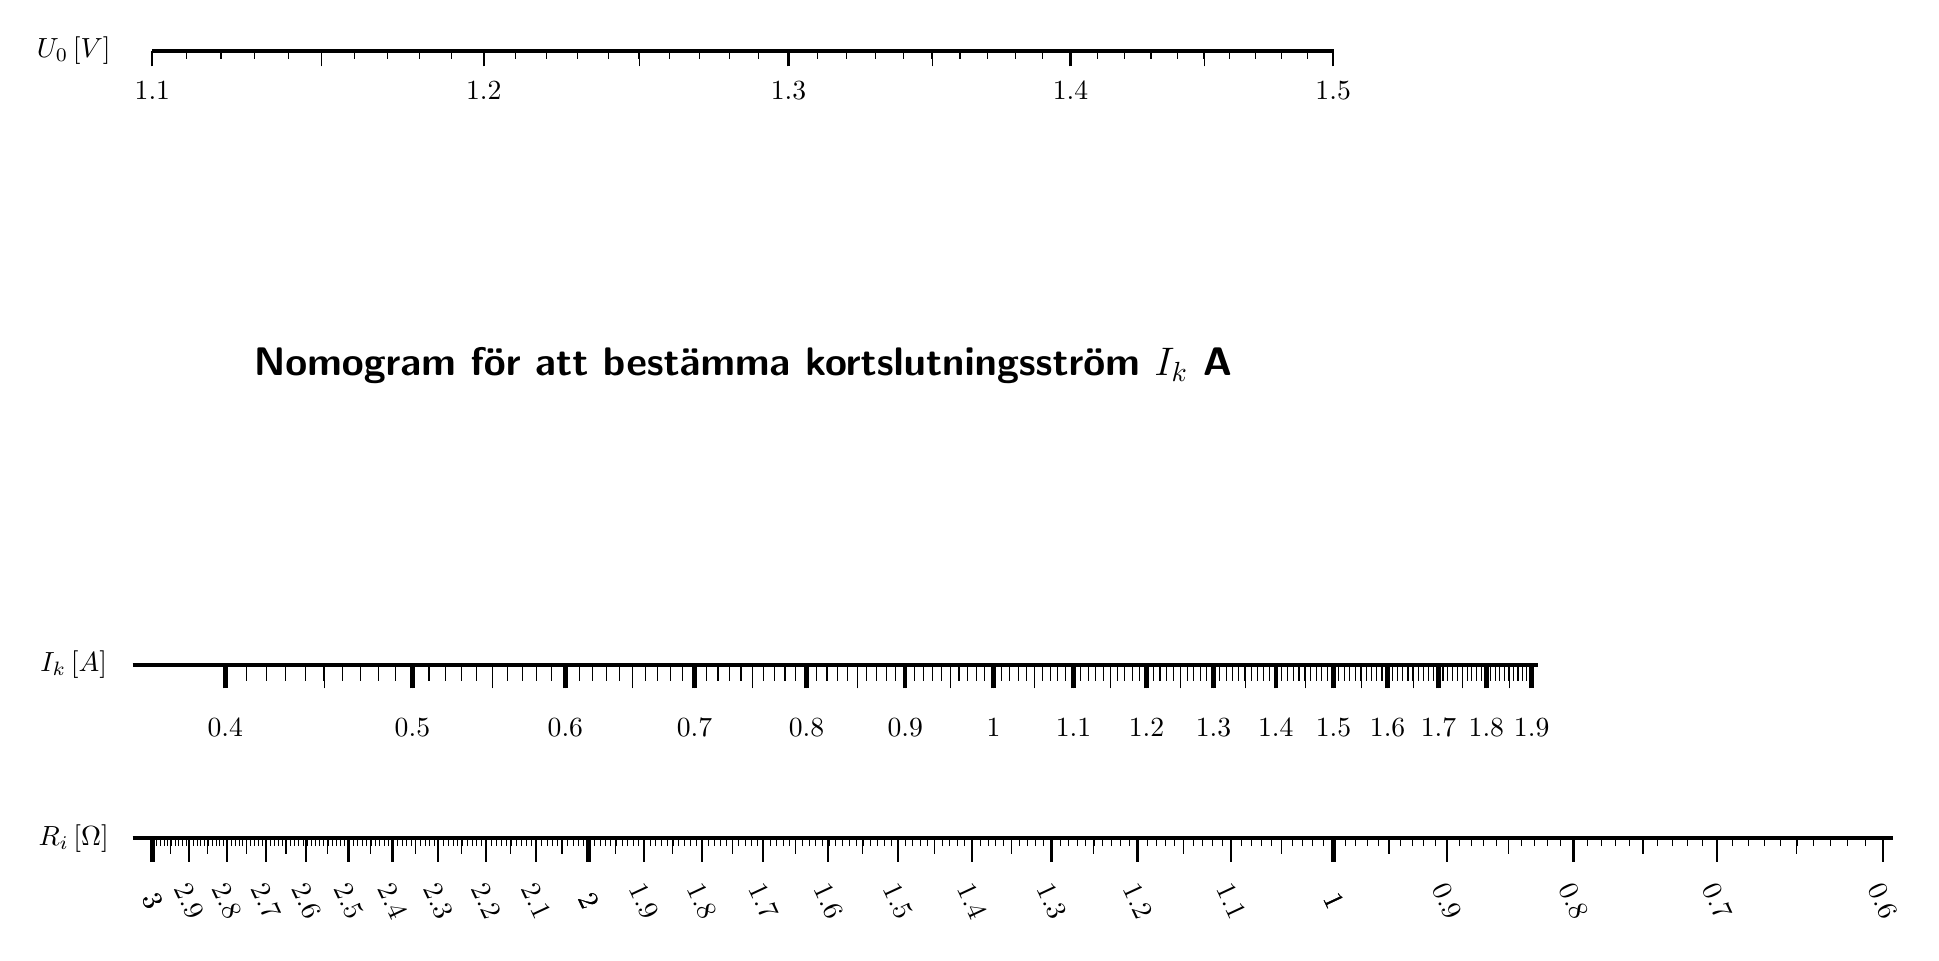
\begin{tikzpicture}[scale=1.0] %[xscale=1.3,yscale=1.3]
%
\draw[ultra thick] (0,0) --(15,0); \node at (-1,0) {$U_0\, [V]$};
% R
\foreach \x in {1.1,1.2,...,1.5} {
\node at (111.35976/ln 10 *ln \x -4.6094, -0.5) {\pgfmathprintnumber[fixed,precision=1]{\x}}; 
\draw[thick] (111.35976/ln 10 *ln \x -4.6094,-0.2) -- (111.35976/ln 10 *ln \x -4.6094,0);
}
\foreach \x in {1.11,1.12,...,1.5} {
\draw[thin] (111.35976/ln 10 *ln \x -4.6094,-0.1) -- (111.35976/ln 10 *ln \x -4.6094,0);
}
\foreach \x in {1.15,1.25,...,1.5} {
\draw[thin] (111.35976/ln 10 *ln \x -4.6094,-0.2) -- (111.35976/ln 10 *ln \x -4.6094,0);
}
\node at (7.5,-4){\Large\textsf{\textbf{Nomogram för att  bestämma kortslutningsström $I_k$ A} }};

% IK
\draw[ultra thick] (-0.25,-7.798) --(17.6,-7.798); 
\node at (-1,-7.798) {$I_k \, [A]$};

\foreach \x in {0.4,0.5,...,1.95} {
\node[rotate=0] at (24.51702/ln 10 *ln \x +10.683, -7.798-0.8) {\pgfmathprintnumber[fixed,precision=1]{\x}}; 
\draw[ultra thick] (24.51702/ln 10 *ln \x +10.683,-7.798-0.3) -- (24.51702/ln 10 *ln \x +10.683,-7.798);
}
\foreach \x in {0.41,0.42,...,1.9} {
\draw[thin] (24.51702/ln 10 *ln \x +10.683,-7.798-0.2) -- (24.51702/ln 10 *ln \x +10.683,-7.798);
}
\foreach \x in {0.45,0.50,...,1.9} {
\draw[thin] (24.51702/ln 10 *ln \x +10.683,-7.798-0.3) -- (24.51702/ln 10 *ln \x +10.683,-7.798);
}

% R_i
\draw[ultra thick] (-0.25,-10) --(22.1,-10); 
\node at (-1,-10) {$R_i \, [\Omega]$};

\foreach \x in {1,2,...,3} {
\node[rotate=-65] at (-31.438/ln 10 *ln \x +15, -10-0.8) {\pgfmathprintnumber[fixed,precision=1]{\x}}; 
\draw[ultra thick] (-31.438/ln 10 *ln \x +15,-10-0.3) -- (-31.438/ln 10 *ln \x +15,-10);
}



%\foreach \x in {1.1,1.2,...,3} {
%\node[rotate=-65] at (-31.438/ln 10 *ln \x +15, -10-0.8) {\pgfmathprintnumber[fixed,precision=1]{\x}};
%\draw[thin] (-31.438/ln 10 *ln \x +15,-10-0.2) -- (-31.438/ln 10 *ln \x +15,-10);
%}
\foreach \x in {1,1.5,...,3} {
\draw[thick] (-31.438/ln 10 *ln \x +15,-10-0.3) -- (-31.438/ln 10 *ln \x +15,-10);
}

\foreach \x in {0.6,0.61,...,3} {
\draw[ultra thin] (-31.438/ln 10 *ln \x +15,-10-0.1) -- (-31.438/ln 10 *ln \x +15,-10);
}
\foreach \x in {0.6,0.65,...,3} {
\draw[ thin] (-31.438/ln 10 *ln \x +15,-10-0.2) -- (-31.438/ln 10 *ln \x +15,-10);
}

\foreach \x in {0.60,0.70,...,3.0} {
\node[rotate=-65] at (-31.438/ln 10 *ln \x +15, -10-0.8) {\pgfmathprintnumber[fixed,precision=2]{\x}};
\draw[thick] (-31.438/ln 10 *ln \x +15,-10-0.3) -- (-31.438/ln 10 *ln \x +15,-10);
}
\end{tikzpicture}
%

\end{document}

